\section{考察}
実験で得られたデータからははっきりと波うつパターンが見て取れる。この章ではその波模様をいくつかの要素に分解し、それぞれについて理論的に説明できるかどうかを考えてゆく。私たちは望んだ干渉の結果を見ることができたのか。

\subsection{波模様の分解$\sim$実験と理論の対応$\sim$}

章で述べたように、干渉パターンは最も一般的には、共鳴からのずれを表すパラメータ$\epsilon$と中性子の速度$v$に依存した係数$N_1,N_2,N_3$を用いて
\begin{equation}
I=N_1-N_2\cos\left(\frac{2}{v}(\omega d'-\epsilon L')\right) -N_3\sin\left(\frac{2}{v}(\omega d'-\epsilon L')\right)
\end{equation}
と表せる。ここで$\omega$は位相シフタコイルの磁場$B_p$を用いて$\omega=|\mu_n|B_p$と表される量であり、$d',L'$はそれぞれ位相シフタコイルの幅、2つのスピンフリッパー間距離である。さらに$N_4=\sqrt{N_2^2+N_3^2}$として
\begin{equation}
\cos \chi=\frac{N_2}{N_4}, \quad \sin \chi=\frac{N_3}{N_4}
\end{equation}
で$\chi$を定義すれば、干渉パターンは
\begin{equation}
I=N_1-N_4\cos\left(\frac{2}{v}(\omega d'-\epsilon L')-\chi\right)
\end{equation}
と書き直される。このように書くと実験データをフィッティングして得られる4つのパラメータと理論式を対応づけることができる。すなわち、実験で得られた波模様を位相シフタコイルに流した電流$I_p$に対して
\begin{equation}
I=D-A\cos(B\cdot I_p+C)
\end{equation}
という関数でフィッティングしたときの4つのパラメータ$A,B,C,D$は理論と
\renewcommand{\arraystretch}{1.5}
\begin{equation}
\begin{array}{l}
A \leftrightarrow N_4\\
B \leftrightarrow \dfrac{2\omega d'}{v(-I_p)}\\
C \leftrightarrow \dfrac{2\epsilon L'}{v} +\chi \\
D \leftrightarrow N_1
\end{array}
\end{equation}
\renewcommand{\arraystretch}{1}
と対応づくことがわかる。なお、$I_p$は鉛直下向きに磁場が発生する向きを正としたため、$B,C$の符号は上のように対応づけるのがよい。

この節の要は、単に実験と理論を対応づけたということではなく、波模様というあいまいな概念を輪郭の明確な4つの要素に分解したことにある。

\subsection{$B$}
\paragraph{パラメータ$B$の特徴}
$B$には干渉という現象のエッセンスが凝縮されている。上では干渉パターンの最も一般的な形を見たが、逆に最も特殊な場合を見てみよう。それは共鳴条件()が満たされている中で、$\pi/2$フリップ条件()を満たす速度の中性子を対象とした場合である。そのときは$N_1=1/2,N_2=1/2,N_3=0,\epsilon=0$であるから、干渉パターンは
\begin{equation}
I=\frac{1}{2}\left(1-\cos\frac{2\omega d'}{v}\right)
\end{equation}
となる。このように、非常にシンプルな場合を考えてもスピン上下の位相差を表す$B$の部分の形は変わらない。そのような意味で$B$は干渉の本質を担っている。

\paragraph{理論からのアプローチ}
理論的には$B$は$2\omega d'/v(-I_p)$と書かれるが、$\omega \propto -I_p$であって、具体的に書けば
\begin{align}
\omega d'&=\frac{|\mu_n|B_p d'}{\hbar} \\ \notag
&=\frac{(-I_p)|\mu_n| b_p d'}{\hbar}
\end{align}
となる。ここで$b_p$は位相シフタコイルに1Aの電流を流したときに発生する磁束密度。なおこの章では実験値と理論値を比較する必要からSI単位系を用い、$\hbar$も明記する。さらに位相シフタコイルによる磁場は空間的に一様ではないため、実際は粒子の軌道に沿って
\begin{equation}
b_p d' \rightarrow \int b_p(x) dx
\end{equation}
と積分で表す必要がある。

次の図\ref{Discussion_fig_PhaseShifterSimulation}は位相シフタコイルに1Aの電流を流したときの磁場分布シミュレーション結果である。またシフタコイルの中心($y=z=0$)を通ったときの$x$軸に沿っての磁場分布を図\ref{Discussion_fig_PSS_danmen}に表す。
\begin{figure}[h]
\begin{minipage}{0.5\hsize}
\centering
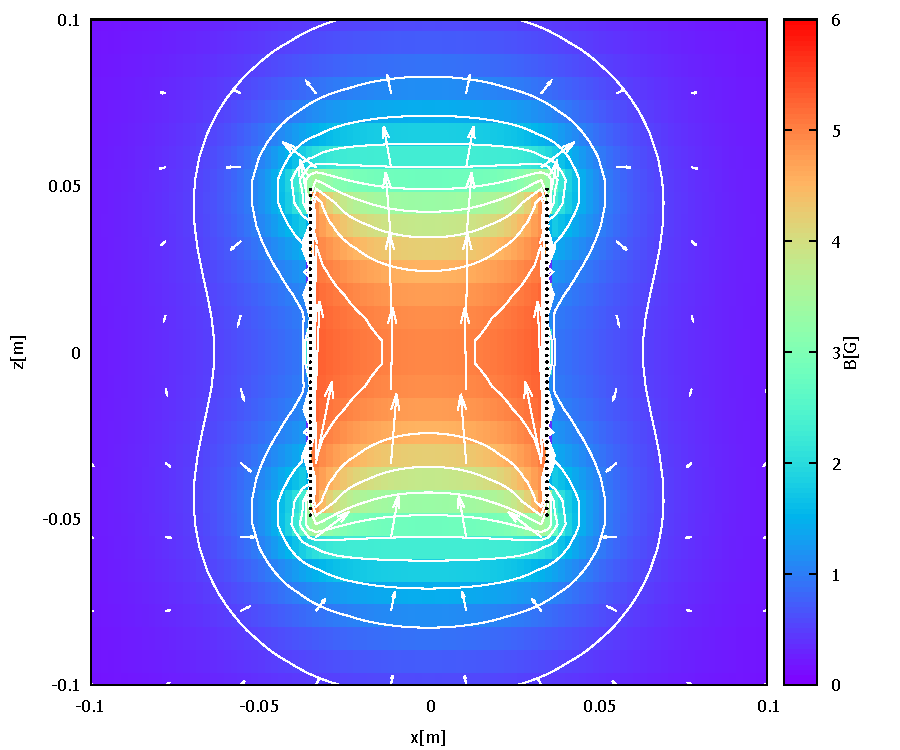
\includegraphics[width=\hsize]{discussion/B/coil11_image1.pdf}
\subcaption{横から}
\end{minipage}
\begin{minipage}{0.5\hsize}
\centering
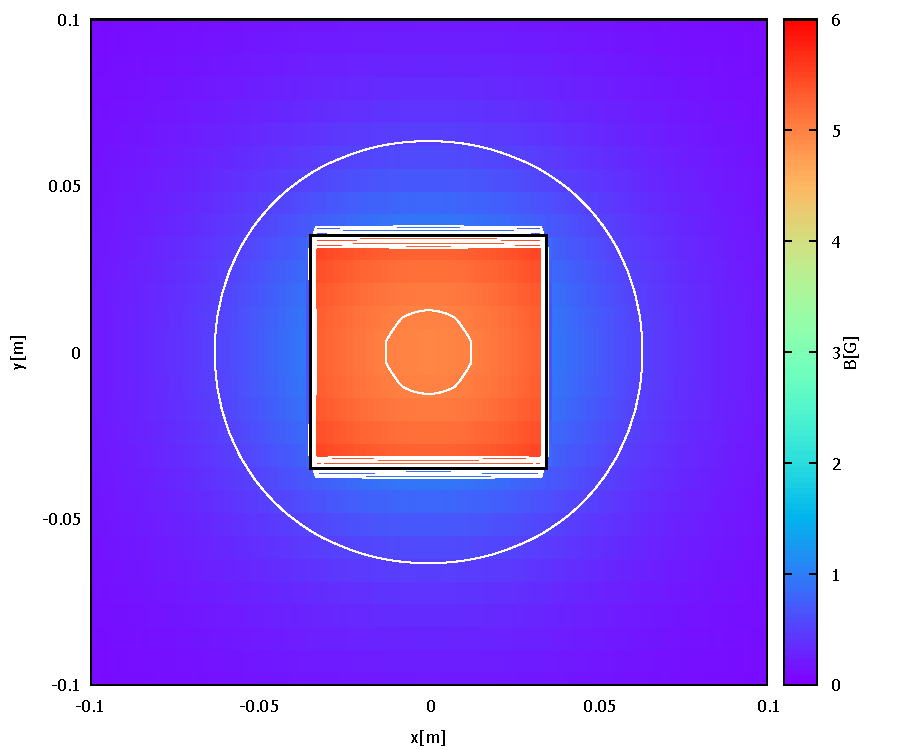
\includegraphics[width=\hsize]{discussion/B/coil11_image2.pdf}
\subcaption{上から}
\end{minipage}
\caption{位相シフタコイル磁場分布シミュレーション} \label{Discussion_fig_PhaseShifterSimulation}
\end{figure}
\begin{figure}[h]
\centering
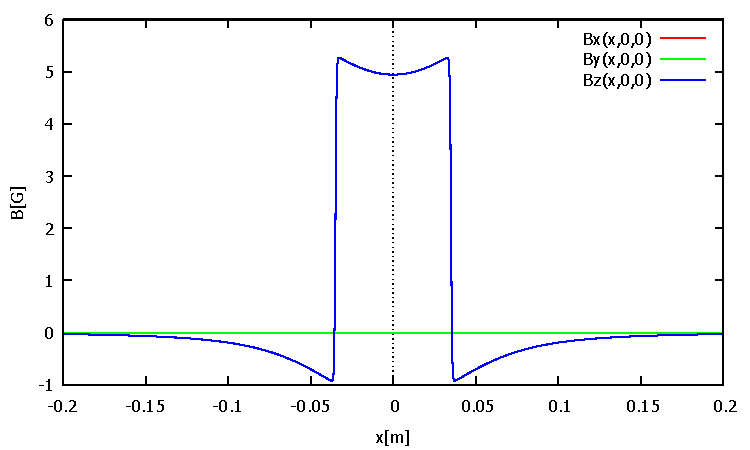
\includegraphics[width=10cm]{discussion/B/coil11_danmen1.pdf}
\caption{$x$軸に沿っての磁場分布シミュレーション} \label{Discussion_fig_PSS_danmen}
\end{figure}

このシミュレーションを用いて$\int b_p(x) dx$を計算すると、シフタコイルの中心($y=z=0$)を通ったときの積分値は
\begin{equation}
\int b_p(x) dx =2.75 \times 10^{-5} \mathrm{T\cdot m/A}
\end{equation}
となった。なお積分範囲は実際の配置と図\ref{Discussion_fig_PSS_danmen}より、$-20$cmから$20$cmとした。また粒子の経路が$y$方向や$z$方向にずれたときの積分値は図\ref{Discussion_fig_PSS_zure}のようになった。ビームの幅は20mm程度であるから、中性子の経路による積分値のずれは1\%程度に抑えられると考えられる。そこで今後の解析には中心での値を用いることにする。
\begin{figure}[h]
\centering
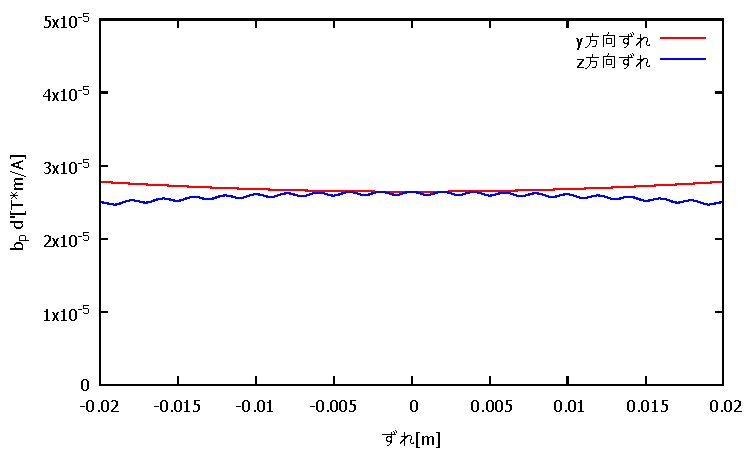
\includegraphics[width=10cm]{discussion/B/bd.pdf}
\caption{$y,z$方向のずれによる影響} \label{Discussion_fig_PSS_zure}
\end{figure}

ゆえに$B$の理論値は
\begin{equation}
\frac{2\omega d'}{v(-I_p)}=2\frac{|\mu_n|\int b_p dx}{\hbar v}=2\frac{|\mu_n|\int b_p dx}{\hbar}\frac{m}{h}\lambda=1.27 \cdot \lambda \ [1/A] \label{Discussion_theory_B}
\end{equation}
となる。ただし$\lambda$[\AA]は中性子の波長。 

\paragraph{実験結果・分析}
以下の表\ref{Discussion_tbl_B}に$\lambda \pm 0.07 \AA$の波長領域において実験データをフィットして得られた$B$の値と式(\ref{Discussion_theory_B})から得られる理論値を示す。なお理論値には中性子の経路による誤差1\% が含まれるとした。また表\ref{Discussion_tbl_B}の結果を図\ref{Discussion_fig_B}に表す。図、表からわかるように全ての波長領域でパラメータ$B$の実験値と理論値はよく一致しており、多くの波長において誤差の範囲で一致している。

\begin{figure}[h]
\begin{minipage}{0.35\hsize}
\centering
\makeatletter
\def\@captype{table}
\makeatother
\caption{各波長領域におけるパラメータ$B$の実験値と理論値} \label{Discussion_tbl_B}
\begin{tabular}{|l|ll|}\hline
$\lambda$[\AA] &  $B(実験)$ &   理論値 \\ \hline
3.06  & 4.18  $\pm$ 0.05  & 3.90  $\pm$ 0.04  \\
3.21  & 4.14  $\pm$ 0.05  & 4.08  $\pm$ 0.04  \\
3.35  & 4.32  $\pm$ 0.05  & 4.27  $\pm$ 0.04  \\
3.42  & 4.42  $\pm$ 0.04  & 4.36  $\pm$ 0.04  \\
3.50  & 4.52  $\pm$ 0.05  & 4.45  $\pm$ 0.04  \\
3.56  & 4.63  $\pm$ 0.07  & 4.54  $\pm$ 0.05  \\
3.66  & 4.74  $\pm$ 0.07  & 4.66  $\pm$ 0.05  \\
3.75  & 4.77  $\pm$ 0.09  & 4.78  $\pm$ 0.05  \\
3.86  & 5.09  $\pm$ 0.09  & 4.91  $\pm$ 0.05  \\
4.00  & 5.15  $\pm$ 0.08  & 5.10  $\pm$ 0.05  \\
4.15  & 5.16  $\pm$ 0.18  & 5.28  $\pm$ 0.05  \\
4.29  & 3.36  $\pm$ 0.17  & 5.47  $\pm$ 0.05  \\ \hline
\end{tabular}
\end{minipage}
\begin{minipage}{0.65\hsize}
\centering
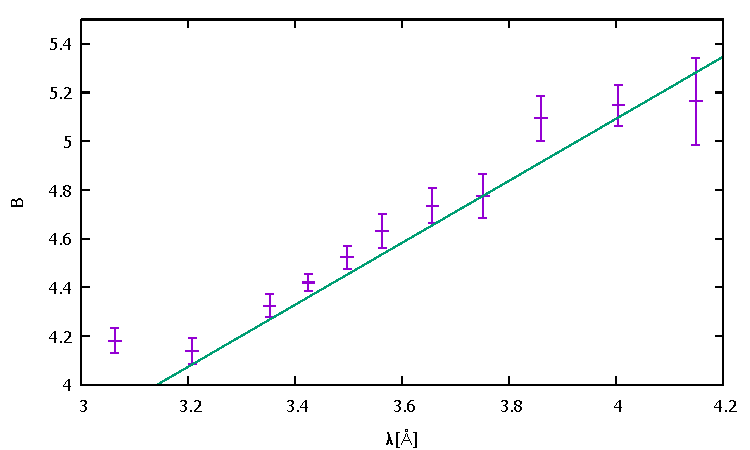
\includegraphics[width=\hsize]{discussion/B/B_F.pdf}
\caption{各波長領域に対する$B$} \label{Discussion_fig_B}
\end{minipage}
\end{figure}

\paragraph{まとめ}
パラメータ$B$こそスピン干渉の本質であり、それが干渉のみられた全ての波長領域で理論値とよく一致したということは、私たちは望みのものを手に入れたということを示唆している。目的は果たされた。




